\documentclass{aa}

\usepackage{graphicx}

\usepackage{txfonts}

\usepackage[hidelinks]{hyperref}

\usepackage{amsmath}

\graphicspath{{./figs/}}

\usepackage{verbatim}

\begin{document} 


   \title{CHEOPS Mission Reduction Pipeline Development}

   \subtitle{Simulation of WASP-18 b - Visit 2}

   \author{João P. S. Rodrigues}

   \institute{Departamento de Física e Astronomia da Universidade do Porto \\
              \email{up201405201@fc.up.pt}              
             }

   \date{}

% \abstract{}{}{}{}{} 
% 5 {} token are mandatory
 
  \abstract
  % context heading (optional)
  % {} leave it empty if necessary  
   {}
  % aims heading (mandatory)
   {}
  % methods heading (mandatory)
   {}
  % results heading (mandatory)
   {}
  % conclusions heading (optional), leave it empty if necessary 
   {}

   \keywords{}

   \maketitle
%
%________________________________________________________________

\section{Introduction}
%__________________________________________________________________

\section{Overscan}

The first step in treating the data is to subtract the overscan values from the image in order to remove the so-called Bias - a systematic error such as electronic noise introduced while reading the CCD .

Since each image is provided with four extra columns of overscan wich contain no data appart from the reading noise, we can use these columns to compute the overscan. By performing an average over each line of the columns and computing the histogram of these average values, we can approximate the noise with a gaussian curve (see Fig. \ref{fig:overscan_hist}). The fit was optimized using the least squares method and the final parameters are $[A, \mu , \sigma] = [9.23, 5260.86, 7.07]$ with one standard deviation errors of $[0.515, 0.455, 0.457]$ respectively.

\begin{figure}
\centering
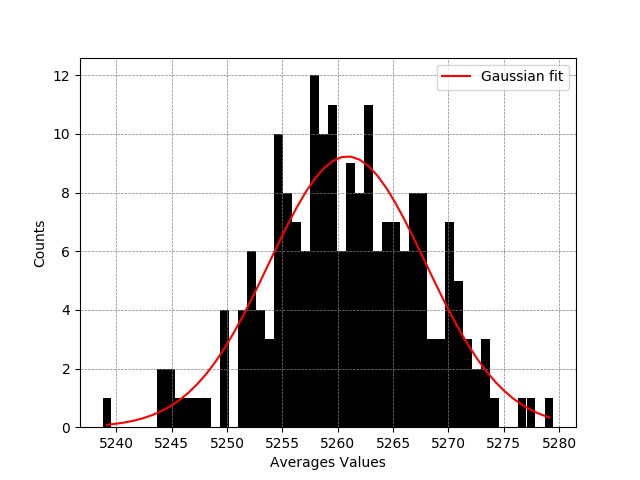
\includegraphics[width=.4\textwidth]{overscan_hist.png}
\caption{Histogram of averages for each line of the 4 columns.}
\label{fig:overscan_hist}
\end{figure}

This allows us to perform an average over all of the four columns and subtract that value from the image data, without introducing significant error.

\section{Flat Field}

The next critical step of the reduction pipeline is to account for the imperfections of the CCD screen when acquiring data. This is done by capturing what is called a Flat Field (FF) image which is the data aquired by the sensor when pointed at a uniform screen.

In order to remove this inconsistent data, the captured images must be divided by the data in the FF image, resulting in an image in which all the CCD pixels have roughly the same sensitivity.

After this step is performed, the pre-processing of the images is complete and one can begin computing the area of the image wherein the target lies, with the objective of performing a photometric measurement.

\section{Center of Mass Calculation}

Taking into account that the order of the counts belonging to the target is much larger than in the rest of the image, one can assume that a rough approximation of the target's position is a computation of the image's center of mass.

However, by computing the center of mass of the whole image, we find that it's position varies in a circular way. This is due to the rotation of the satellite together with the other objects which very faintly appear in the images. These objects are better observed by computing a convolution of the image with a Scharr Kernel of the type:

\begin{equation}
\begin{bmatrix}

-3-3j  & 0-10j &  +3 -3j \\
-10+0j & 0+ 0j & +10 +0j \\
-3+3j  & 0+10j &  +3 +3j

\end{bmatrix}
\end{equation}

which computes the gradient of the image both in magnitude and direction. The direction of the image's gradient is shown in Fig. \ref{fig:gradient_cm} (a) where the existence of at least three other objects, besides the target, is made obvious. We can also notice that these objects are rotating around the target in a clockwise manner which explains the circular movement of the images' center of mass, seen in Fig. \ref{fig:gradient_cm} (b).

\begin{figure}
\centering

(a) 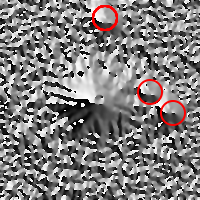
\includegraphics[width=.2\textwidth]{gradient_angle_img_0.png}
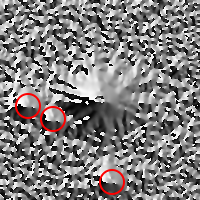
\includegraphics[width=.2\textwidth]{gradient_angle_img_45.png}

(b) 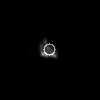
\includegraphics[width=.2\textwidth]{cm_r_100_img_0.png}
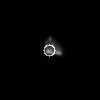
\includegraphics[width=.2\textwidth]{cm_r_100_img_45.png}

(c) 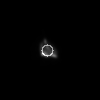
\includegraphics[width=.2\textwidth]{cm_r_20_img_0.png}
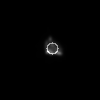
\includegraphics[width=.2\textwidth]{cm_r_20_img_45.png}
\caption{From top to bottom: (a) Direction of the images' gradient.
							  (b) Center of mass calculated using the whole image.
							  (c) Center of mass calculated using a square of size 20 pixels 									 centered on the images' center.}
\label{fig:gradient_cm}
\end{figure}

As a means to fix this problem, the center of mass was calculated using a square centered on the images' center and of a radius $r_{CM}$ to be empirically computed in Sec. \ref{sec:param_opt}. This way, the calculation only envolves the target and not the other objects, thus improving the stability of the center of mass, which can be seen in Fig. \ref{fig:gradient_cm} (c).

\section{Canny Edge Detection}

From observing the images in Fig. \ref{fig:gradient_cm} (a), an idea arised to use the gradient of the images to find the region on which to perform the photometry. An obvious candidate for an algorithm popped into mind: Canny Edge Detection \cite{canny}. The algorithm has the following steps:

\begin{enumerate}
\item Apply Gaussian filter to remove noise.
\item Compute intensity gradient of the image.
\item Apply non-maximum surpression.
\item Apply double threshold to determine edges.
\item Edge tracking by hysteresis.
\end{enumerate}

Even though this is the standard procedure to perform the canny edge algorithm, we can disregard the third step since applying the surpression is just an edge-thining technique which is of no use for us since we want to find the area inside the outer edges, anyway.

The same principle (used in the calculation of the center of mass) of applying the algorithm to a box centered on the image was utilized here in order to find only the edges of the target. As such, this algorithm, if correctly applied - using optimized parameters of filter $\sigma$ and double thresholds, discussed in Sec. \ref{sec:param_opt} - should return the area of the target in a specific image.

As can be seen in Fig. \ref{fig:img_0_canny}, the algorithm seems to be a good candidate for detecting the target's area, for as much as can be seen with the naked eye. This figure was obtained with $\sigma = 0.6$, higher threshold $T = 4000$ and lower threshold $t = 0.3T$.

\begin{figure}
\centering

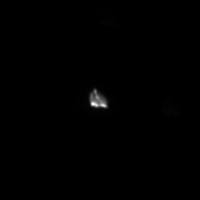
\includegraphics[width=.2\textwidth]{img_0.png}
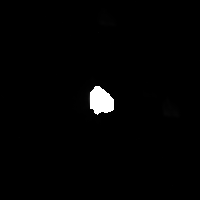
\includegraphics[width=.2\textwidth]{img_0_canny.png}

\caption{Comparison of image 0 target with detected area.}
\label{fig:img_0_canny}
\end{figure}




\section{Photometry}

\section{Parameter Optimization} \label{sec:param_opt}

\section{Timing Optimization}


%                                     Two column figure (place early!)
%______________________________________________ Gamma_1 (lg rho, lg e)
%   \begin{figure*}
%   \centering
   %%%\includegraphics{empty.eps}
   %%%\includegraphics{empty.eps}
   %%%\includegraphics{empty.eps}
%   \caption{Adiabatic exponent $\Gamma_1$.
%               $\Gamma_1$ is plotted as a function of
%               $\lg$ internal energy $\mathrm{[erg\,g^{-1}]}$ and $\lg$
%               density $\mathrm{[g\,cm^{-3}]}$.}
%              \label{FigGam}%
%    \end{figure*}
%

%
%                                                One column figure
%----------------------------------------------------------- S_vib
%   \begin{figure}
%   \centering
   %%%\includegraphics[width=3cm]{empty.eps}
%      \caption{Vibrational stability equation of state
%               $S_{\mathrm{vib}}(\lg e, \lg \rho)$.
%               $>0$ means vibrational stability.
%              }
%         \label{FigVibStab}
%   \end{figure}
%
%______________________________________________________________

\section{Conclusions}

%   \begin{enumerate}
%      \item conclusion 1
%      \item conclusion 2
%   \end{enumerate}

%\begin{acknowledgements}
%      Part of this work was supported by the German
%      \emph{Deut\-sche For\-schungs\-ge\-mein\-schaft, DFG\/} project
%      number Ts~17/2--1.
%\end{acknowledgements}

% WARNING
%-------------------------------------------------------------------
% Please note that we have included the references to the file aa.dem in
% order to compile it, but we ask you to:
%
% - use BibTeX with the regular commands:
%   \bibliographystyle{aa} % style aa.bst
%   \bibliography{Yourfile} % your references Yourfile.bib
%
% - join the .bib files when you upload your source files
%-------------------------------------------------------------------

\begin{thebibliography}{}

\bibitem[(Canny 1986)]{canny} Canny, J. 1986,
      in IEEE Transactions on Pattern Analysis and Machine Intelligence

\end{thebibliography}

\end{document}